\section{Simulations and program evaluation}\label{sec:experiments}

\subsection{Simulations}

\begin{figure}[ht]
\begin{centering}
     \begin{subfigure}[b]{0.48\textwidth}
         \centering
         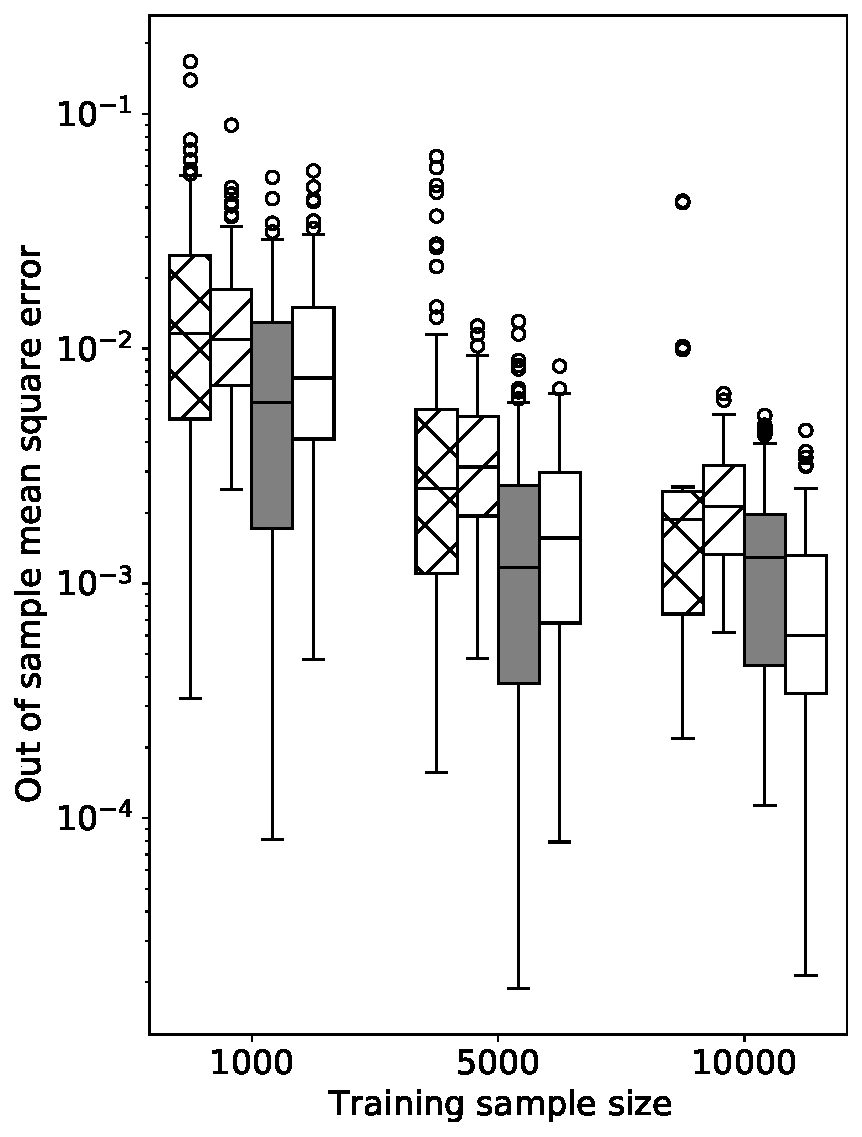
\includegraphics[width=\textwidth]{img/colangelo_all2_sub_rep100_all_bma.pdf}
         %\vspace{-20pt}
         \caption{Dose response curve.}
     \end{subfigure}
     \hfill
     \begin{subfigure}[b]{0.48\textwidth}
         \centering
         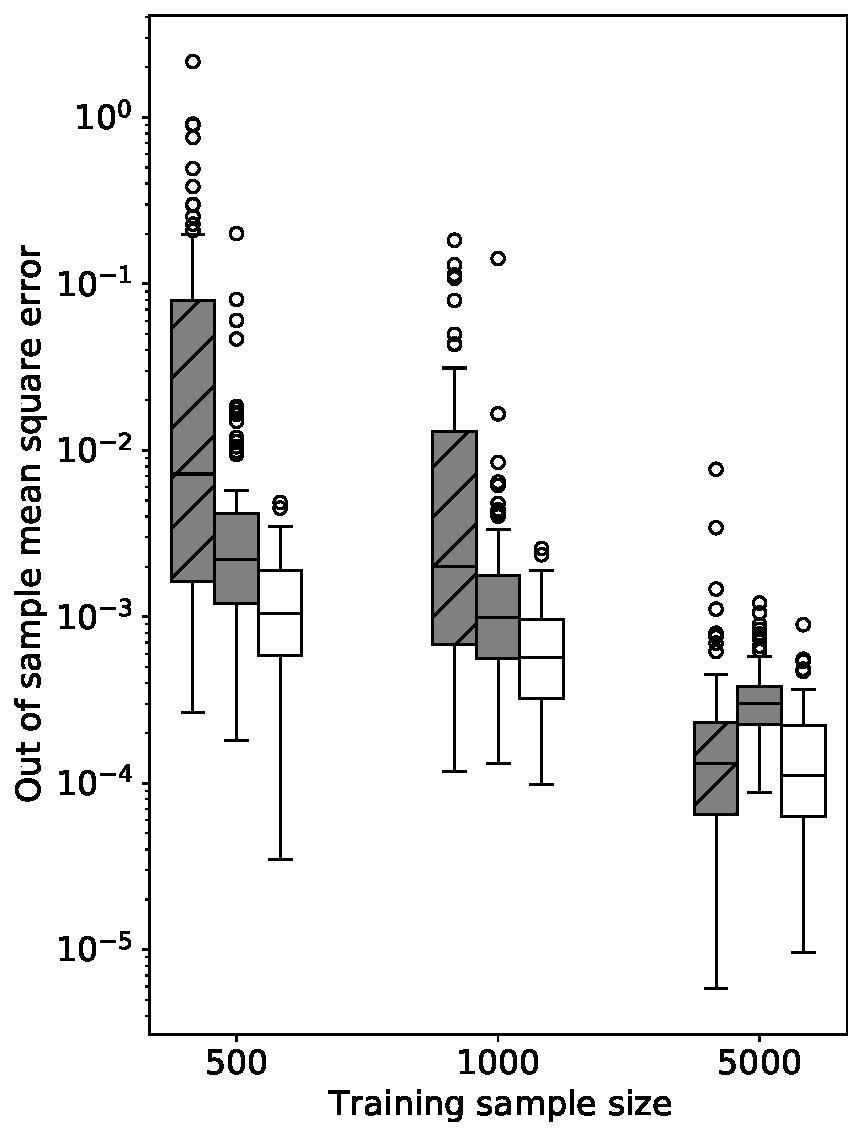
\includegraphics[width=\textwidth]{img/CATE_synthetic2_rep100_all_bma.pdf}
         %\vspace{-20pt}
         \caption{Heterogeneous treatment effect.}
     \end{subfigure}
\par
%\vspace{-10pt}
\caption{\label{fig:cont}
Nonparametric causal function simulations. We implement the estimators of \cite{abrevaya2015estimating} (\texttt{IPW}, lined gray), \cite{kennedy2017nonparametric} (\texttt{DR1}, checkered white), \cite{colangelo2020double} (\texttt{DR2}, lined white), and \cite{semenova2021debiased} (\texttt{DR-series}, gray), in addition to our own (\texttt{RKHS}, white).}
\end{centering}
\end{figure}
We demonstrate that our nonparametric causal function estimators outperform some leading alternatives in nonlinear simulations with many covariates, despite the relative simplicity of our proposed approach. For each causal function design and sample size, we implement 100 simulations and calculate mean square error with respect to the true causal function. Figure~\ref{fig:cont} visualizes results. A lower mean square error is desirable. See Supplement~\ref{sec:simulations} for a full exposition of the data generating processes and implementation details.  

The dose response curve design \cite{colangelo2020double} involves learning the causal function $\theta_0^{ATE}(d)=1.2d+d^2$. A single observation consists of the triple $(Y,D,X)$ for outcome, treatment, and high dimensional covariates where $Y,D\in\mathbb{R}$ and $X\in\mathbb{R}^{100}$. In addition to our one-line nonparametric estimator (\texttt{RKHS}, white), we implement the estimators of \cite{kennedy2017nonparametric} (\texttt{DR1}, checkered white), \cite{colangelo2020double} (\texttt{DR2}, lined white), and \cite{semenova2021debiased} (\texttt{DR-series}, gray). \texttt{DR1} and \texttt{DR2} are local estimators that involve Nadaraya--Watson smoothing around doubly robust estimating equations. \texttt{DR-series} uses series regression with debiased pseudo outcomes, and we give it the advantage of correct specification as a quadratic function. By the Wilcoxon rank sum test, \texttt{RKHS} significantly outperforms alternatives at sample size 10,000, with p value less than $10^{-3}$, despite its relative simplicity.

Though our approach allows for heterogeneous response of a continuous treatment, we implement a design for heterogeneous effect of a binary treatment in order to facilitate comparison with existing methods. The heterogeneous treatment effect design \cite{abrevaya2015estimating} involves learning the causal functions $\theta_0^{CATE}(0,v)=0$ and $\theta_0^{CATE}(1,v)=v(1+2v)^2(v-1)^2$. A single observations consists of the tuple $(Y,D,V,X)$ for outcome, treatment, covariate of interest, and other covariates. In this design, $Y,D,V\in\mathbb{R}$ and  $X\in\mathbb{R}^3$. In addition to our one-line nonparametric estimator (\texttt{RKHS}, white), we implement the estimators of \cite{abrevaya2015estimating} (\texttt{IPW}, lined gray) and \cite{semenova2021debiased} (\texttt{DR-series}, gray). The former involves Nadaraya--Watson smoothing around an inverse propensity estimator, and the latter involves (correctly specified) series regression with a debiased pseudo outcome. The R learner \cite{nie2021quasi} cannot be implemented since $V\neq X$. The simple \texttt{RKHS} approach significantly outperforms alternatives at sample sizes 500 and 1,000 by the Wilcoxon rank sum test, with p values less than $10^{-5}$. 
\subsection{Program evaluation: US Job Corps}


\begin{figure}[ht]
\begin{centering}
     \begin{subfigure}[b]{0.45\textwidth}
         \centering
         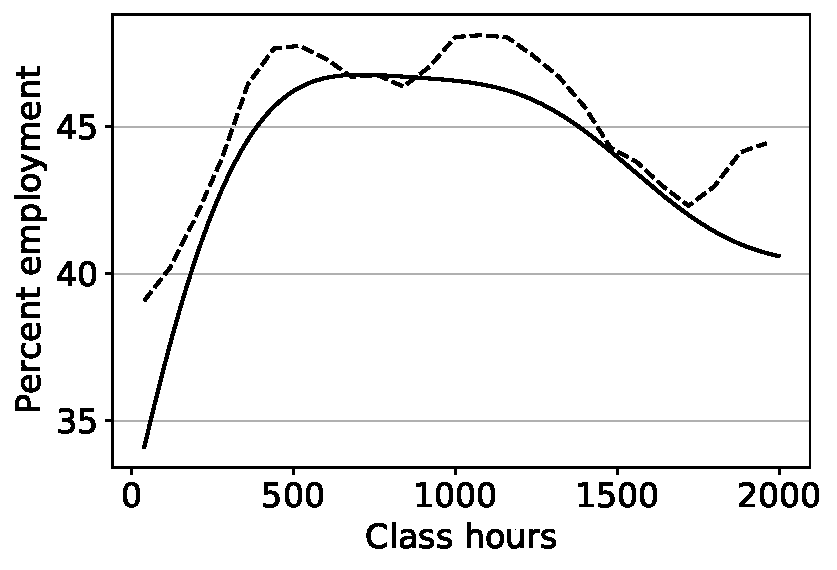
\includegraphics[width=\textwidth]{img/ATE_JCdata_d_filter_with_dml_bma.pdf}
         %\vspace{-20pt}
         \caption{Dose response curve.}
     \end{subfigure}
     \hfill
     \begin{subfigure}[b]{0.45\textwidth}
         \centering
         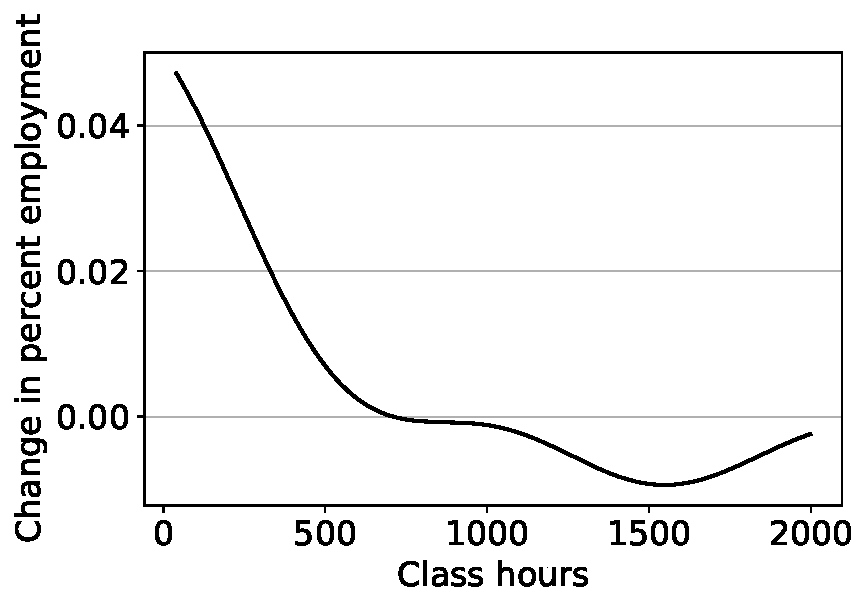
\includegraphics[width=\textwidth]{img/Incremental_ATE_JCdata_d_filter_bma.pdf}
         %\vspace{-20pt}
         \caption{Incremental response curve.}
     \end{subfigure}
     %\vskip\baselineskip
     \begin{subfigure}[b]{0.45\textwidth}
         \centering
         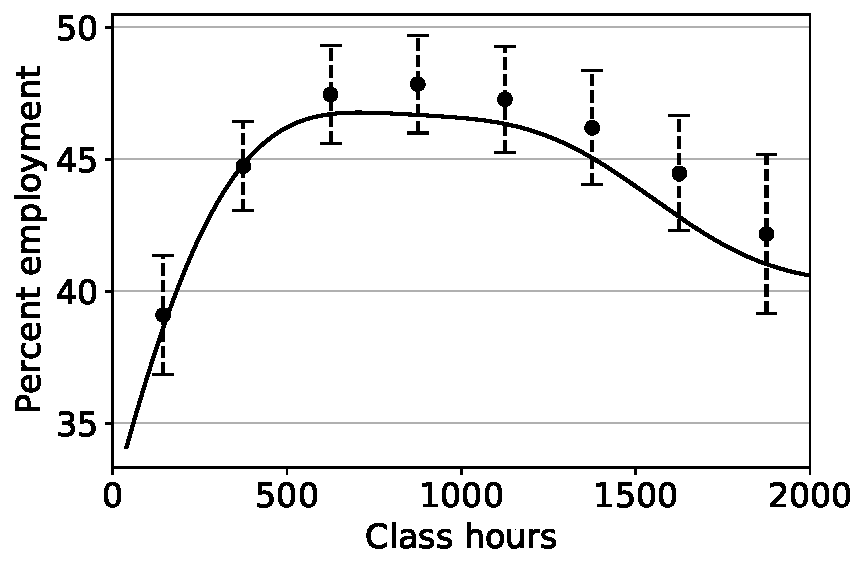
\includegraphics[width=\textwidth]{img/ATE_JCdata_d_filter_ci_fine_gaussian2_bma.pdf}
         %\vspace{-20pt}
         \caption{Discrete treatment effects.}
     \end{subfigure}
     \hfill
     \begin{subfigure}[b]{0.45\textwidth}
         \centering
         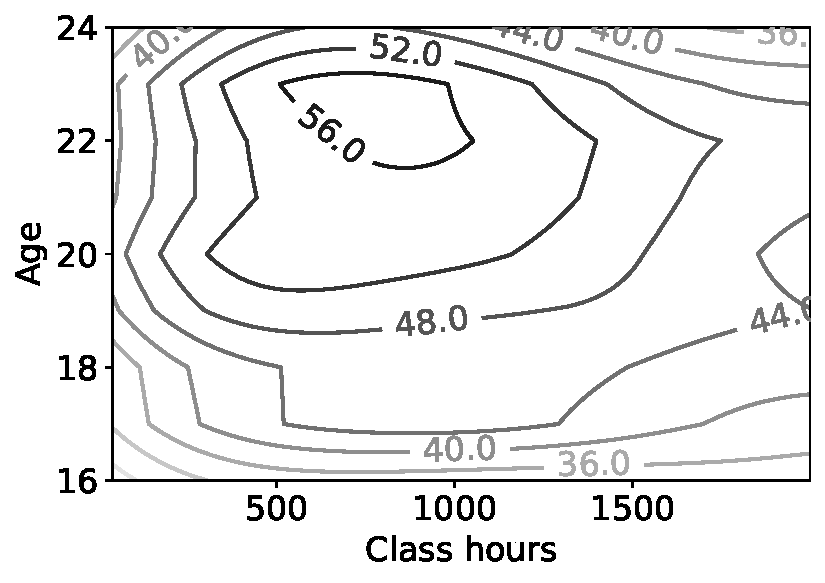
\includegraphics[width=\textwidth]{img/CATE_Age_JCdata_d_filter_bma.pdf}
         %\vspace{-20pt}
         \caption{Heterogeneous response curve.}
     \end{subfigure}
\par
%\vspace{-10pt}
\caption{\label{fig:JC}
Effect of job training on employment. We implement our estimators for dose, heterogeneous, and incremental response curves (\texttt{RKHS}, solid). For comparison, we also implement the dose response curve estimator of \cite{colangelo2020double} (\texttt{DR2}, dashes) as well as the discrete treatment effects of \cite{singh2021debiased} (\texttt{DR3}, vertical bars).}
\end{centering}
\end{figure}

To demonstrate how kernel methods for causal functions are a practical addition to the empirical economic toolkit, we conduct a real world program evaluation. Specifically, we estimate dose, heterogeneous, and incremental response curves of the Jobs Corps, the largest job training program for disadvantaged youth in the US. The Job Corps is financed by the US Department of Labor, and it serves about 50,000 participants annually. Participation is free for individuals who meet low income requirements. Access to the program was randomized from November 1994 to February 1996; see \cite{schochet2008does} for details. Many studies focus on data from this period to evaluate the effect of job training on employment \cite{flores2012estimating,colangelo2020double}. Though access to the program was randomized, individuals could decide whether to participate and for how many hours. From a causal perspective, we assume selection on observables: conditional on observed covariates, participation was exogenous on the extensive and intensive margins. From a statistical perspective, we assume that different intensities of job training have smooth effects on counterfactual employment, and that those effects are smoothly modified by age, assumptions motivated by labor market theory.

In this setting, the continuous treatment $D\in\mathbb{R}$ is total hours spent in academic or vocational classes in the first year after randomization, and the continuous outcome $Y\in\mathbb{R}$ is the proportion of weeks employed in the second year after randomization. The covariates $X\in\mathbb{R}^{40}$ include age, gender, ethnicity, language competency, education, marital
status, household size, household income, previous receipt of social aid, family background, health, and health related behavior at base line. As in \cite{colangelo2020double}, we focus on the $n=3,906$ observations for which $D\geq 40$, i.e. individuals who completed at least one week of training. We implement various causal parameters in Figure~\ref{fig:JC}: the dose response curve; the incremental response curve; the discrete treatment effects with confidence intervals of \cite{singh2021debiased}; and the heterogeneous response curve with respect to age. For the discrete effects, we discretize treatment into roughly equiprobable bins: $[40,250]$, $(250,500]$, $(500,750]$ $(750,1000]$, $(1000,1250]$, $(1250,1500]$, $(1500,1750]$, and $(1750,2000]$ class hours. As far as we know, the heterogeneous response of class hours, a continuous treatment, has not been previously studied in this empirical setting. In Supplement~\ref{sec:application}, we provide implementation details and verify that our results are robust to the choice of sample.

The dose response curve plateaus and achieves its maximum around $d=500$, corresponding to 12.5 weeks of classes. Our global estimate (\texttt{RKHS}, solid) has the same overall shape but is smoother and slightly lower than the collection of local estimates from \cite{colangelo2020double} (\texttt{DR2}, dashes). The smoothness of our estimator is a consequence of the RKHS assumptions, and we see how it is a virtue for empirical economic research; a smooth dose response curve is more economically plausible in this setting. The first 12.5 weeks of classes confer most of the gain in employment: from 35\% employment to more than 47\% employment for the average participant. The incremental response curve (\texttt{RKHS}, solid) is the derivative of the dose response curve, and it visualizes where the greatest gain happens. The discrete treatment effects of \cite{singh2021debiased} (\texttt{DR3}, vertical bars) corroborate our dose response curve, and the 95\% confidence intervals contain the dose response curve of \cite{colangelo2020double} (\texttt{DR2}, dashes) as well as our own (\texttt{RKHS}, solid). 
%By measuring continuous treatment effects rather than binary treatment effects, we are able to determine how many class hours are optimal. 
Finally, the heterogeneous response curve (\texttt{RKHS}, solid) shows that age plays a substantial role in the effectiveness of the intervention. For the youngest participants, the intervention has a small effect: employment only increases from 28\% to at most 36\%. For older participants, the intervention has a large effect: employment increases from 40\% to 56\%. %Again, the first 12 weeks of classes confer the greatest gain. By measuring heterogeneous treatment effects, we are able to determine the subpopulation for whom class hours are most effective. 
Our policy recommendation is therefore 12--14 weeks of classes targeting individuals 21--23 years old.
